
\chapter{Results and Discussion}

The simulator capture sets of five perspective images and converts them into one image, mimicking the effect of fisheye lenses cameras. Using the setup described in Section~\ref{sec:combining_pictures}, and an calibratable polynomial lens model, each images is mapped onto specific parts of the final fisheye image. In Figure~\ref{fig:res_show_fisheye} the complete image is shown, simulating a $270^\circ$ FoV camera mounted beneath the multirotor during flight. The simulator is fully implemented for Linux, but will work on Windows with some modifications to the build system and client program. This includes removing the ROS publisher, as ROS is currently not available on Windows platforms. No part of the simulator has been tested on Mac OS. 

\begin{figure}[!htb]
    \centering
    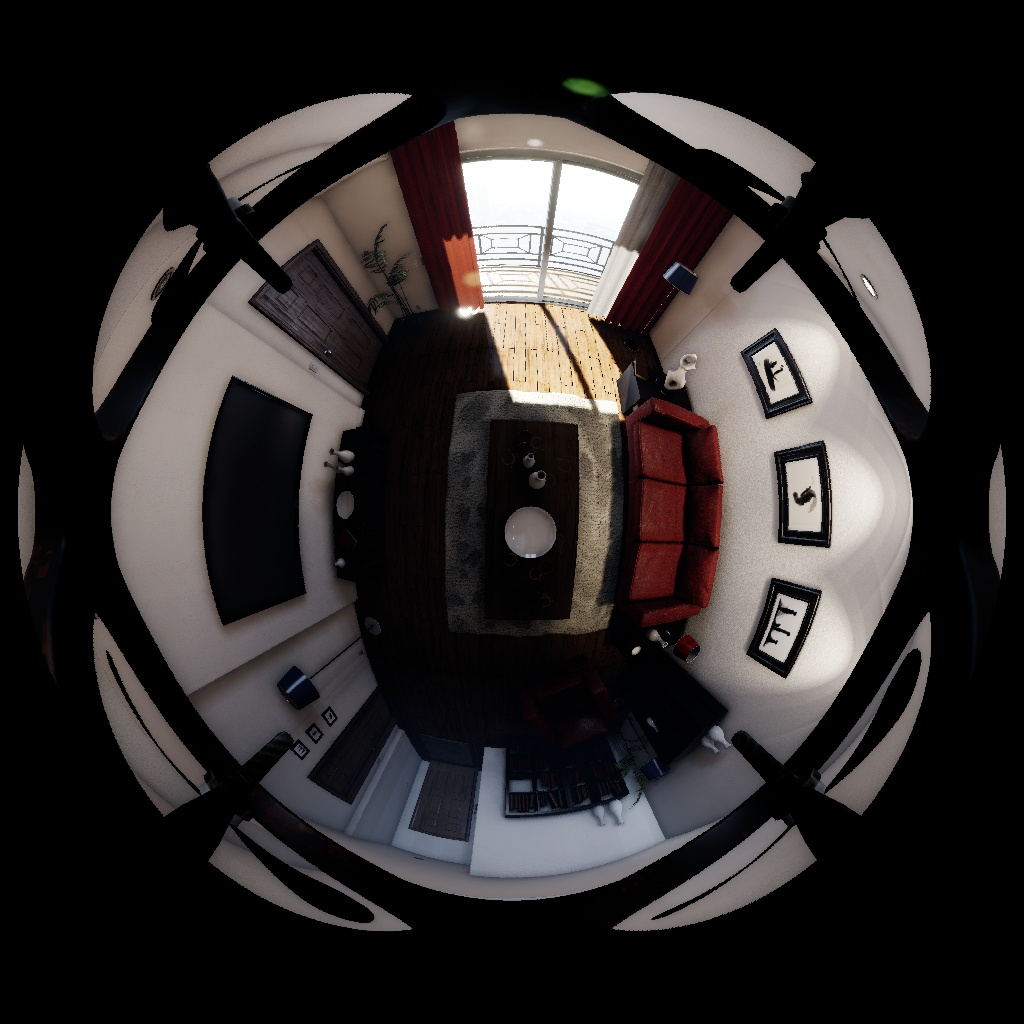
\includegraphics[width=0.7\textwidth]{rapport/fig/Results/1024to1024.jpeg}
    \caption{Simulated fisheye image taken in an indoor environment in Unreal Engine}
    \label{fig:res_show_fisheye}
\end{figure}

\section{Results} \label{sec:Results}

The simulator is able to capture either single $90^\circ$ Fov pictures or full $270^\circ$ FoV pictures. This is because the simulator assumes the full five-camera setup, if it receives more than one image for transformation. The single pictures may be taken by any of the five cameras. This is donw by changing the image request sent to AirSim and setting the cameraposition as down, which tells the tranformer that the image does not need to be rotated.

The resolution settings for the perspective images can be set to a maximum of $4096\times4096$, and while there is no current limit to the resolution of the fisheye image, the height and width should should not exceed the double of the input image sizes. The FOV must equal $90^\circ$ for cube capture, but can be both increased and decreased for single captures, as long as the aspect ratio is preserved. 

\subsection{Fisheye captures and capture environment}

The images was taken in a indoor evironment provided by the Unreal Engine scene library. This is one of the freely available scenes in the Unreal Engine Library, and provides different types of lighting, some reflecting surfaces, as well as enough objects to be able to test the image quality. In Figure~\ref{fig:res_inflight} an inflight picture of the scene can be seen, while Figure~\ref{fig:res_original_pictures} shows five pictures taken from the multirotor through AirSim. These images are taken with the default camera effect settings, which has a fast working auto exposure and no motion blur added. Picture noise is also tuned off.

\begin{figure}[!htb]
    \centering
    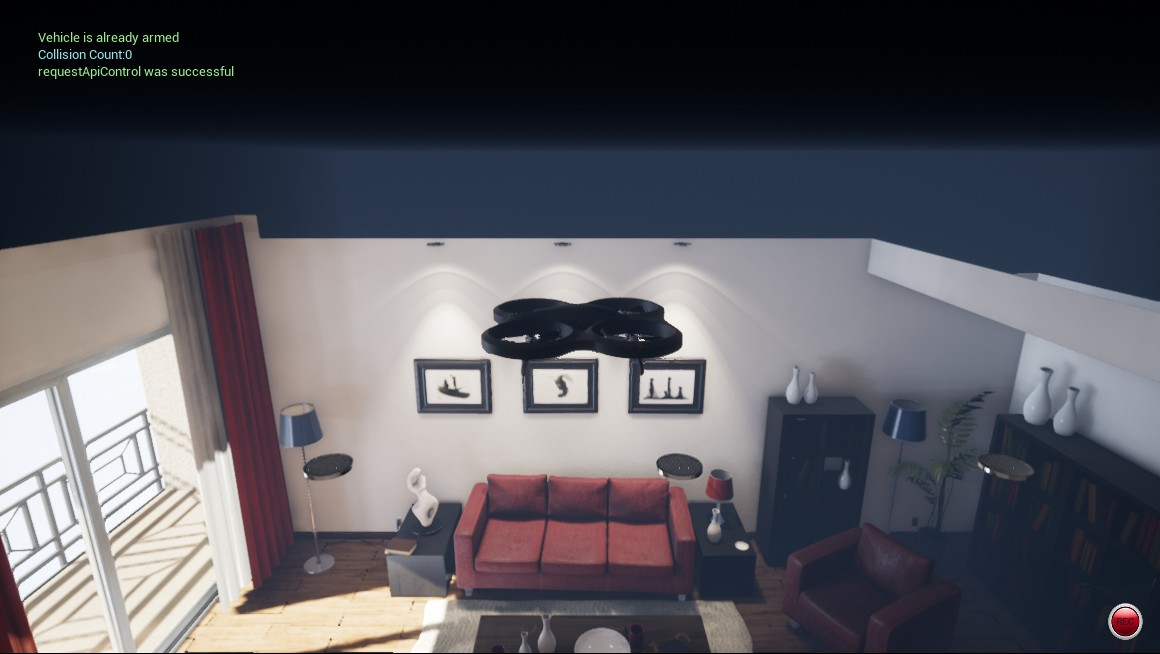
\includegraphics[width = 0.7\textwidth]{rapport/fig/Results/inflight.jpg}
    \caption{Indoor test scene in the Unreal Engine editor}
    \label{fig:res_inflight}
\end{figure}

The simulator will work in any environment created in Unreal Engine, by adding the project specific files along the AirSim files to the new scene. Figure \todo[inline]{add new environment} shows the same simulator in two other environments. The process of using pre-made scenes may be a bit tedious for Linux, since most scenes has been created for Windows. However, Unreal Engine provides tools for converting the projects to support Linux, and as of now all scenes have worked.

\begin{figure}[!htb]
    \centering
    \begin{subfigure}{0.32\textwidth}
    \centering
        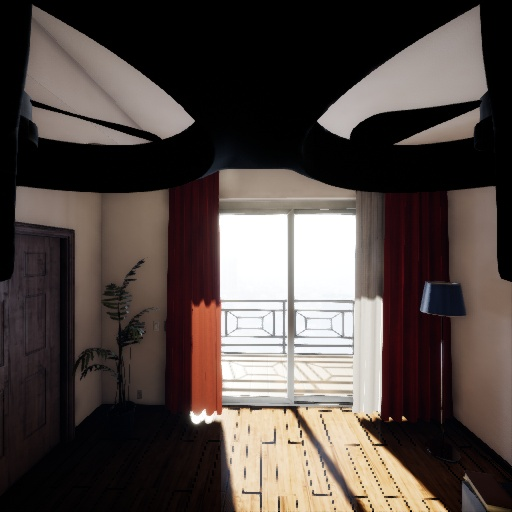
\includegraphics[height=5cm]{rapport/fig/Results/single/forward_center.jpeg}
        \caption{Front Camera}
        \label{fig:res_original_front}
    \end{subfigure}
    \begin{subfigure}{0.32\textwidth}
        \centering
        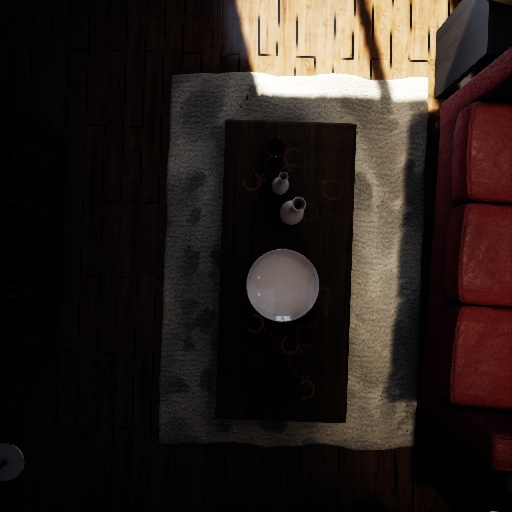
\includegraphics[height=5cm]{rapport/fig/Results/single/down_center.jpeg}
        \caption{Downward camera}
        \label{fig:res_original_down}
    \end{subfigure}    
    \begin{subfigure}{0.32\textwidth}
        \centering
        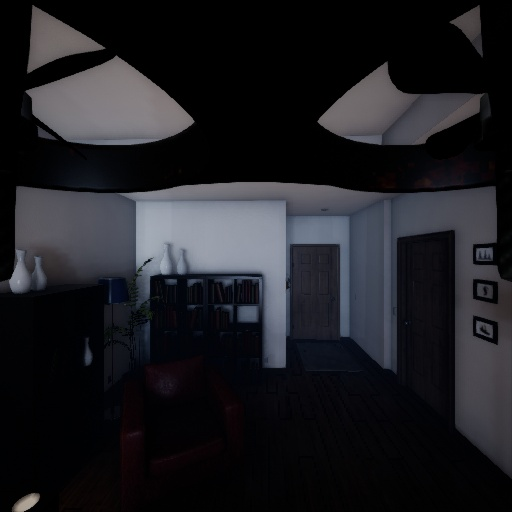
\includegraphics[height=5cm]{rapport/fig/Results/single/backward_center.jpeg}
        \caption{Back camera}
        \label{fig:res_original_back}
    \end{subfigure} \\[0.75ex]
    \begin{subfigure}{0.32\textwidth}
        \centering
        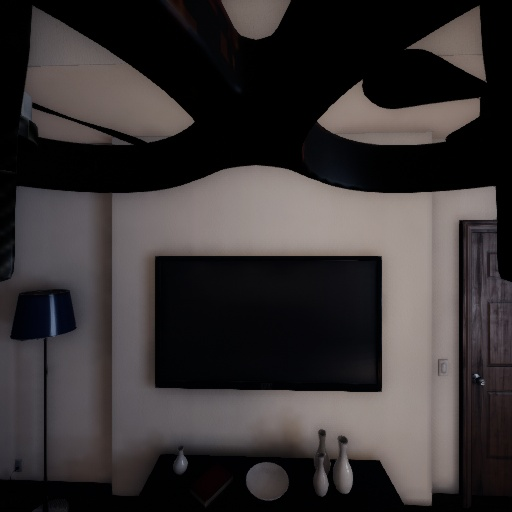
\includegraphics[height=5cm]{rapport/fig/Results/single/left_center.jpeg}
        \caption{Left Camera}
        \label{fig:res_original_left}
    \end{subfigure}
    \begin{subfigure}{0.32\textwidth}
        \centering
        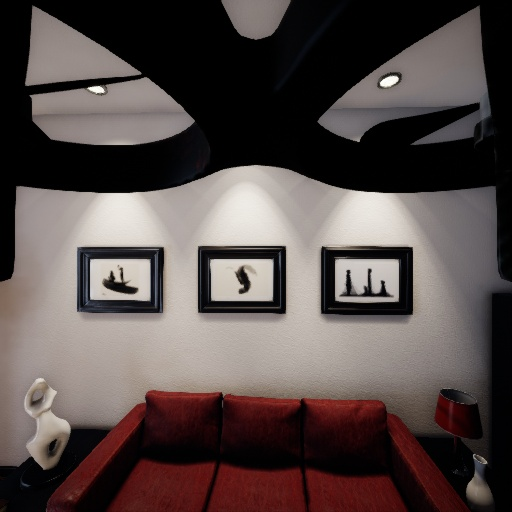
\includegraphics[height=5cm]{rapport/fig/Results/single/right_center.jpeg}
        \caption{Right Camera}
        \label{fig:res_original_right}
    \end{subfigure}
    \centering
    \caption{The original perspective images from Airsim, taken in flight}
    \label{fig:res_original_pictures}
\end{figure}

\subsection{Cube capture and omnidirectional fisheye iamge tranformation}

The perspective images seen in ~\ref{fig:res_original_pictures} were taken were taken from the air, as shown in Figure~\ref{fig:res_inflight}. Since these cameras cover a $360^\circ$ horizontal FoV and a $270^\circ$ vertical FoV, they also capture parts of the multirotor the camera cluster is attatched to. These features will be apparent in the transformed pictures shown later in the section.

Figure~\ref{fig:res_quality_comparison} shows three images taken with different resolution, and using an equiangular projection. The resolution in the compared pictures matches that of the perspective image resolution. This means that the $512\times512$ pixel image is combined from five $512\times512$ pixel images and so on. One can see that the image in Figure~\ref{fig:res_comp_256_to_256} is substantially lower than that of the image in Figure~\ref{fig:res_comp_1024_1024}. Almost all details on the door and railing are lost, and the reflection seen in the plate at the table is almost none existent. Comparing Figure~\ref{fig:res_comp_512_512} and Figure~\ref{fig:res_comp_1024_1024}, the differences are quite minimal.

\begin{figure}[!htb]
    \centering
    \begin{subfigure}{0.45\textwidth}
    \centering
        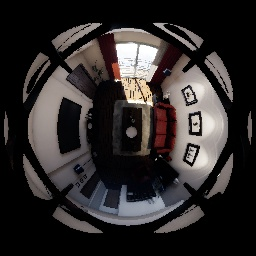
\includegraphics[height=6cm]{rapport/fig/Results/256to256.jpeg}
        \caption{$256 \times 256$ pixels}
        \label{fig:res_comp_256_to_256}
    \end{subfigure}
    \begin{subfigure}{0.45\textwidth}
        \centering
        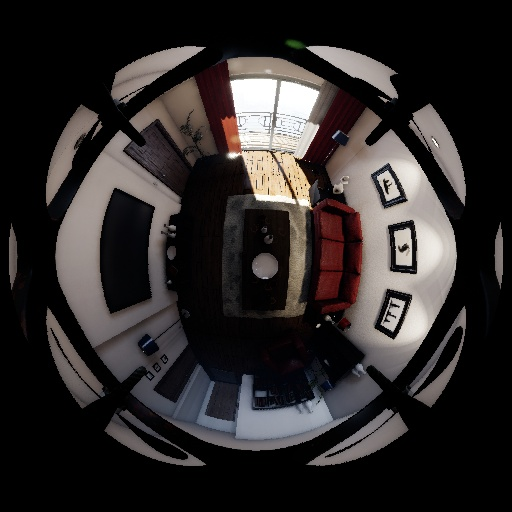
\includegraphics[height=6cm]{rapport/fig/Results/512to512.jpeg}
        \caption{$512 \times 512$ pixels}
        \label{fig:res_comp_512_512}
    \end{subfigure} \\   
    \begin{subfigure}{0.7\textwidth}
        \centering
        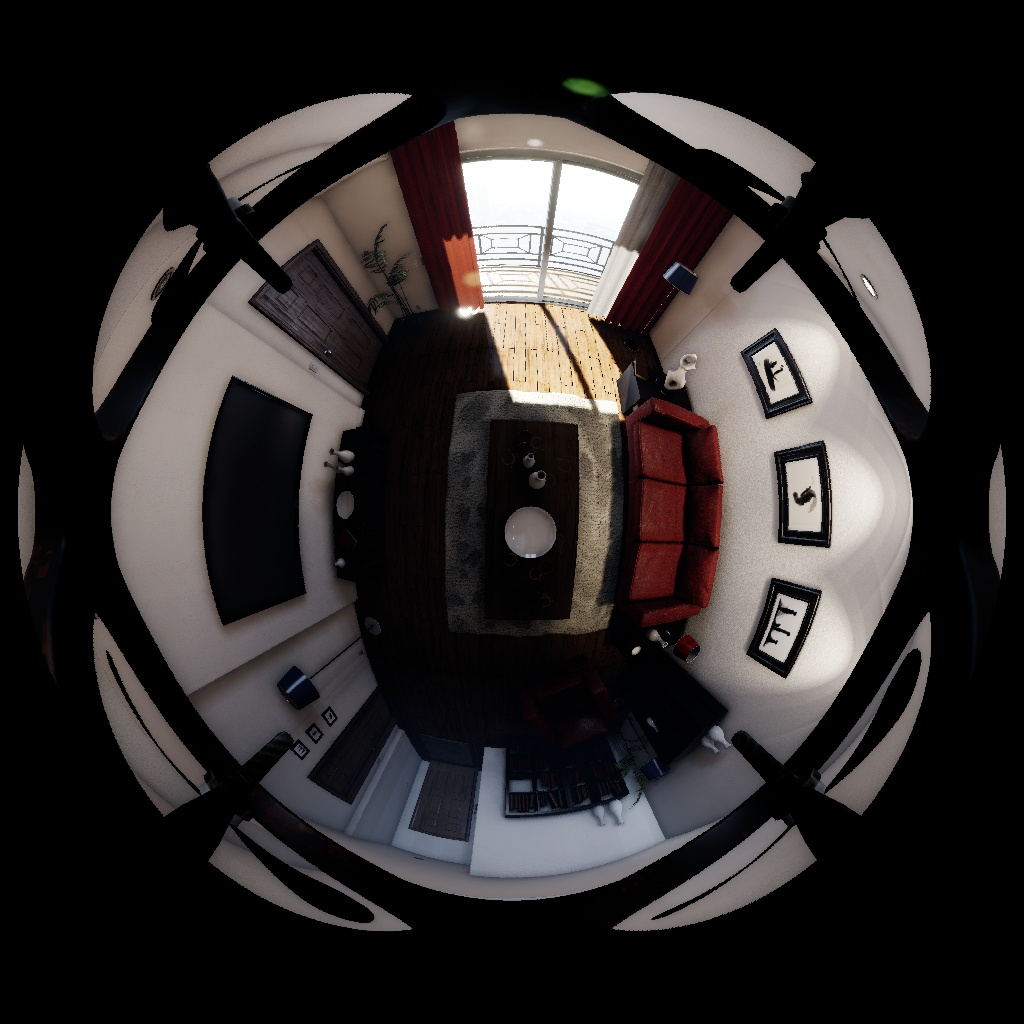
\includegraphics[height=6cm]{rapport/fig/Results/1024to1024.jpeg}
        \caption{$1024 \times 1024$ pixels}
        \label{fig:res_comp_1024_1024}
    \end{subfigure}
    \centering
    \caption{Image quality comparison, where that resolution and of the output picture matches the resolution of the five perspective images}
    \label{fig:res_quality_comparison}
\end{figure}

The images in Figure~\ref{fig:res_comp_equal} are taken with the same perspective image resolution of $512 \times 512$, but with two different destination resolutions. The most important difference here is the distortion lines seen in Figure~\ref{fig:res_comp_equal_512_1024}, caused by the stretching of the source image. However, it can also be seen that the detail level in the central parts have been increased.

\begin{figure}[!htb]
    \centering
    \begin{subfigure}{0.45\textwidth}
        \centering
        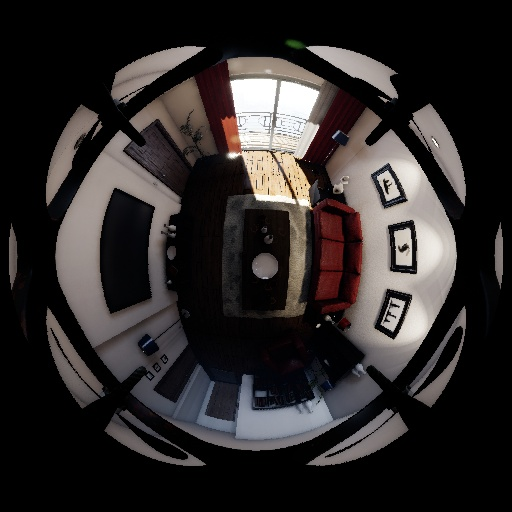
\includegraphics[height=6cm]{rapport/fig/Results/512to512.jpeg}
        \caption{$512 \times 512$ pixels}
        \label{fig:res_comp_equal_512_512}
    \end{subfigure}
    \begin{subfigure}{0.45\textwidth}
        \centering
        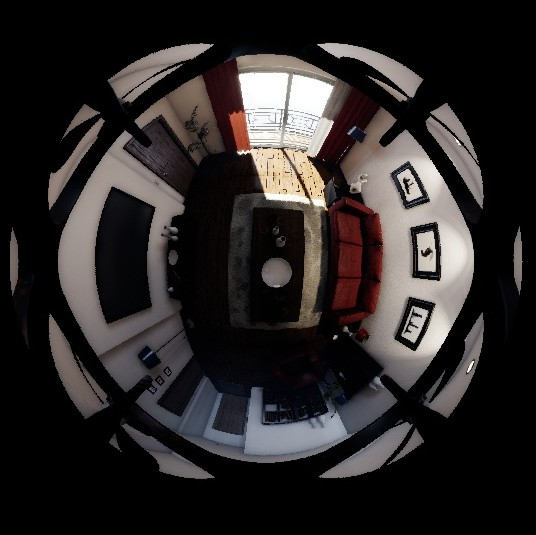
\includegraphics[height=6cm]{rapport/fig/Results/512to1024.jpeg}
        \caption{$1024 \times 1024$ pixels}
        \label{fig:res_comp_equal_512_1024}
    \end{subfigure}
    \caption{Comparison of images transformed from five $512 \times 512$ pixel perspective images}
    \label{fig:res_comp_equal}
\end{figure}

Adding noise and changing exposure settings is integrated into AirSim, and is set in the AirSim settings. Figure~\ref{fig:res_pp} shows three images, where \ref{fig:res_pp_noise_yes} has added noise, both in the form of random pixel intensity and in the form of flickering, noise lines and distortion. The effects have been exagerated to make it visible in the report. All effects can be controlled independently. One thing to note is that these effects are applied to the perspective images. This means that they will be distorted by the fisheye transformer after this effect is applied. This adds extra smudging, especially at higher $\phi$ values. 

\begin{figure}[!htb]
    \centering
    \begin{subfigure}{0.45\textwidth}
        \centering
        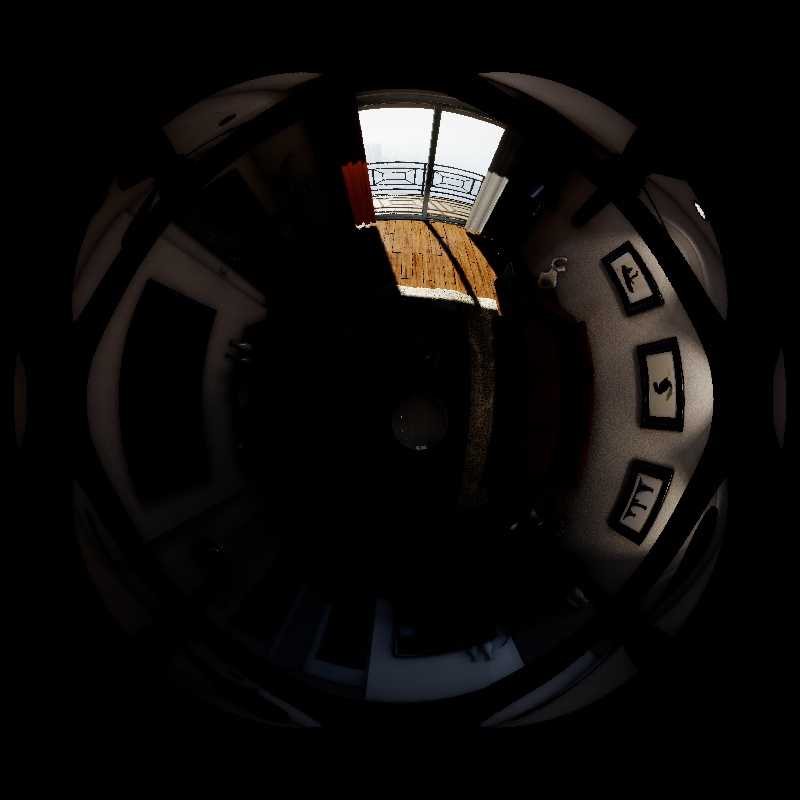
\includegraphics[height=6cm]{rapport/fig/Results/pp/no_nooise_high_min_brightness.jpeg}
        \caption{Low exposure time}
        \label{fig:res_pp_exposure_yes}
    \end{subfigure}
    \begin{subfigure}{0.45\textwidth}
        \centering
        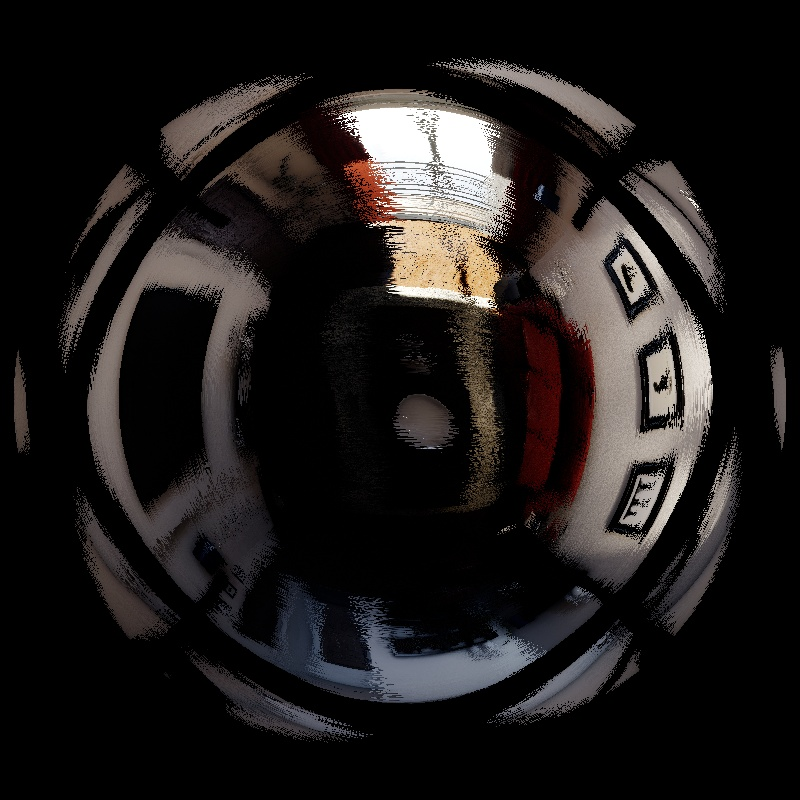
\includegraphics[height=6cm]{rapport/fig/Results/pp/noise_normal_exposure.jpeg}
        \caption{Noisy picture}
        \label{fig:res_pp_noise_yes}
    \end{subfigure}
    \caption{Additional noise and exposure added to the image}
    \label{fig:res_pp}
\end{figure}

Figure~\ref{fig:res_pp_exposure_yes} has had it's exposure massively reduced, and this is also an effect directly integrated by AirSim. The settings allow the user to control the amount of automatic exposure adjustment speed, as well as maximum and minimum values. This effect has been nicely integrated into the fisheye-transformed image, without any apparent side effects. There are manual controls for this in Unreal Engine, but they have not been transferred to AirSim's settings. This is however controlable from the editor directly.

\subsection{Single picture distortion}

Figure~\ref{fig:res_comp_single} shows how single pictures are distorted using the same equidistant lens model. These picture were taken from the front camera on the multirotor, while stationary on the table. The most noticable effect in this picture is the effect the direct sunlight has on the exposure. This makes the rest of the scene appear much darker, which is a normal effect seen in cameras. At low resolutions there are unfortunately some texture clipping, especially of the plant in Figrue~\ref{fig:res_comp_single_256_200}.

\begin{figure}[!htb]
    \centering
    \begin{subfigure}{0.45\textwidth}
        \centering
        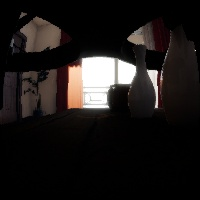
\includegraphics[height=6cm]{rapport/fig/Results/single/single_256_200.jpeg}
        \caption{$200 \times 200$ pixels}
        \label{fig:res_comp_single_256_200}
    \end{subfigure}
    \begin{subfigure}{0.45\textwidth}
        \centering
        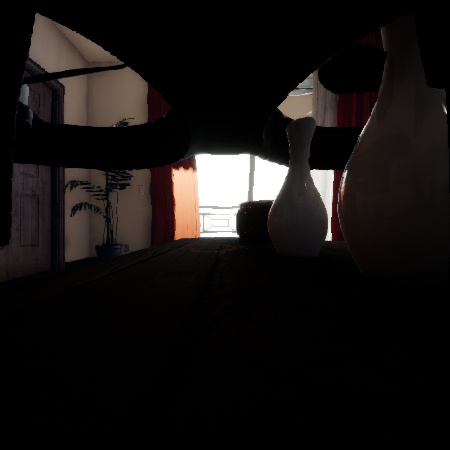
\includegraphics[height=6cm]{rapport/fig/Results/single/single_512_450.jpeg}
        \caption{$450 \times 450$ pixels}
        \label{fig:res_comp_single_512_450}
    \end{subfigure} \\

    \begin{subfigure}{0.45\textwidth}
        \centering
        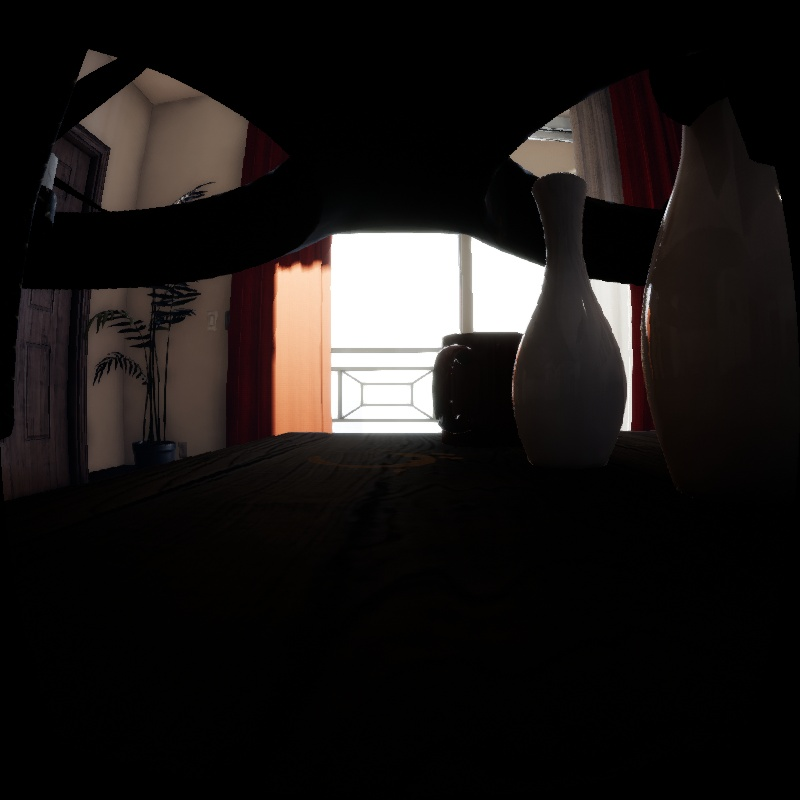
\includegraphics[height=6cm]{rapport/fig/Results/single/single_1024_800.jpeg}
        \caption{$800 \times 800$ pixels}
        \label{fig:res_comp_single_1024_800}
    \end{subfigure}
    \begin{subfigure}{0.45\textwidth}
        \centering
        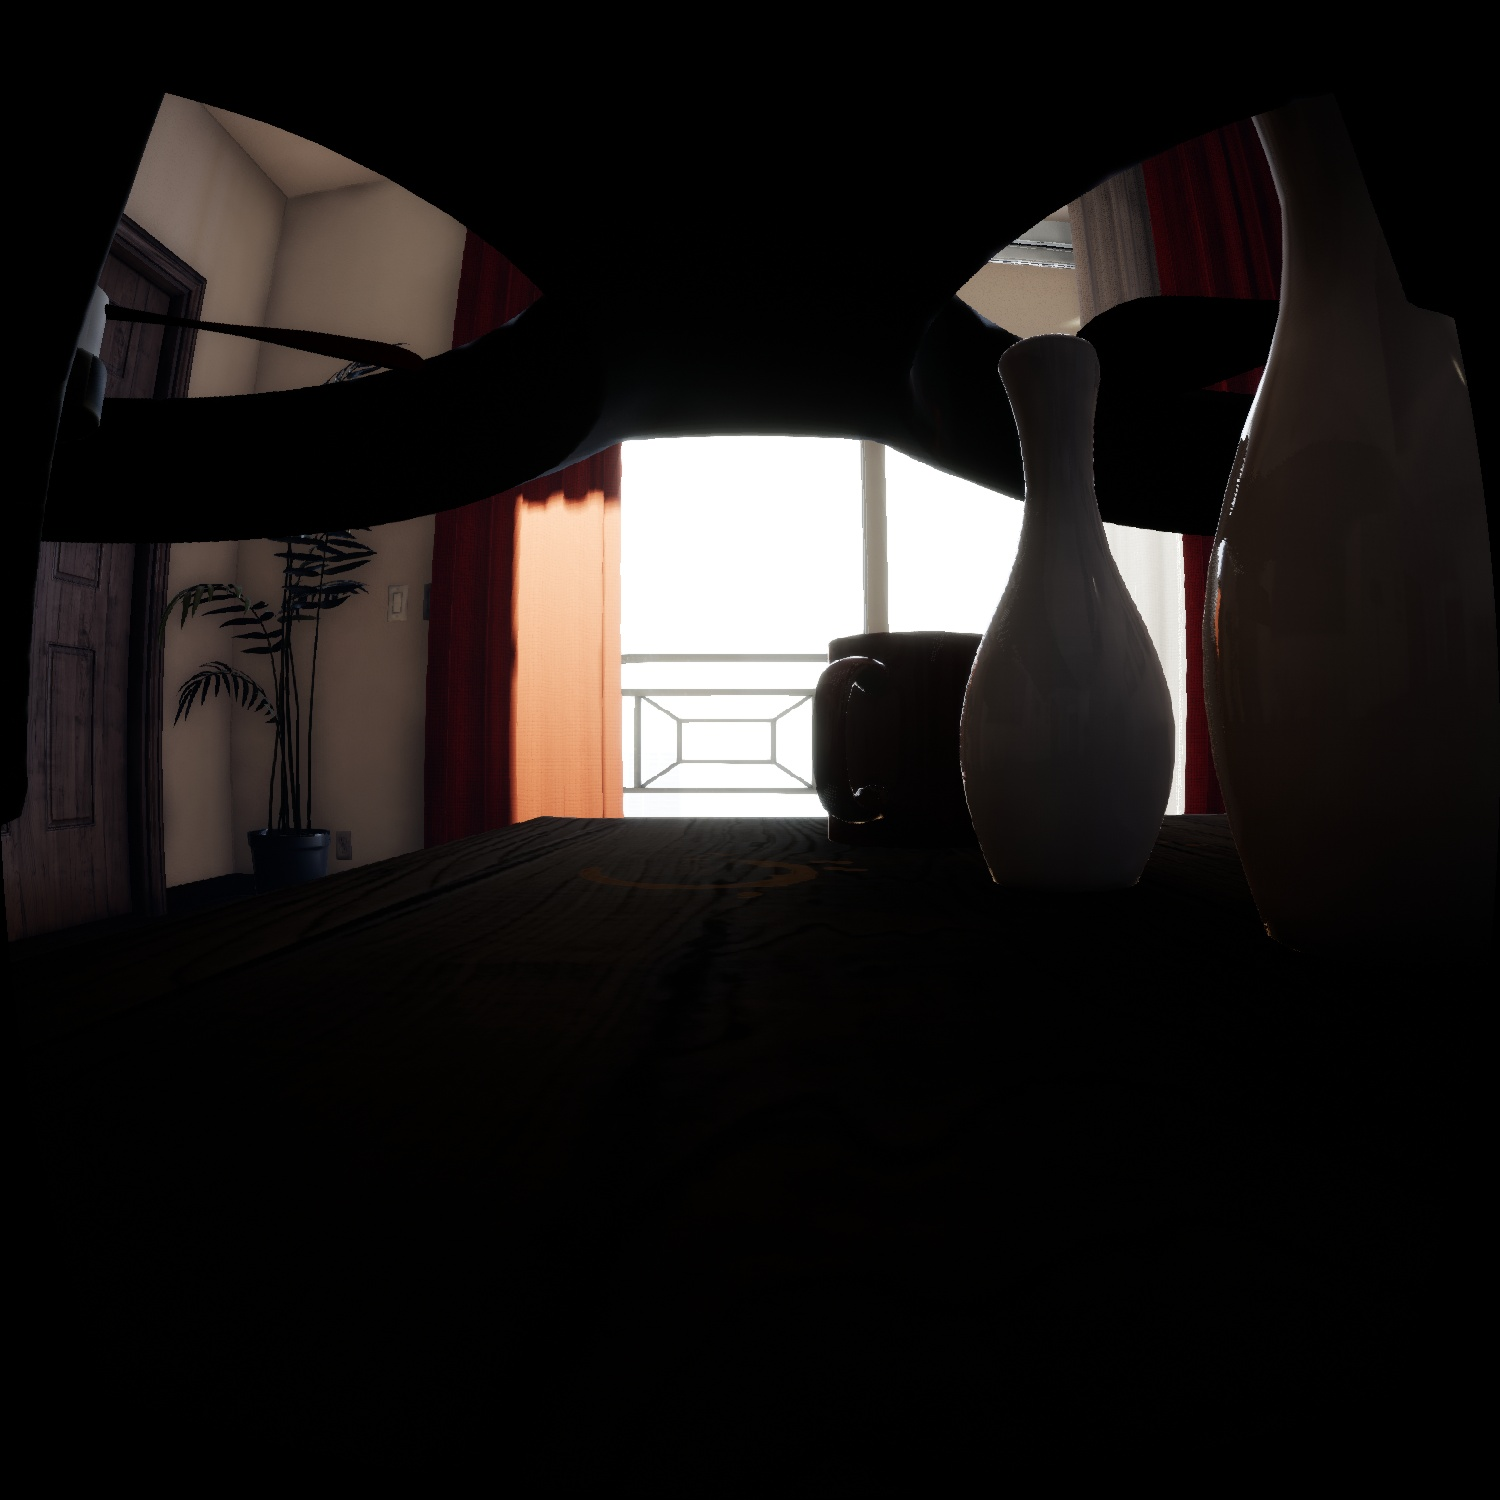
\includegraphics[height=6cm]{rapport/fig/Results//single/single_2048_1500.jpeg}
        \caption{$1500 \times 1500$ pixels}
        \label{fig:res_comp_single_2048_1500}
    \end{subfigure}
    \caption{Transformed images taken based on a single perspective image at different resolutions}
    \label{fig:res_comp_single}    
\end{figure}

The simulator also allows altering of the distortion model. This can be seen in Figure~\ref{fig:res_different_distortions}, where three distortion models are presented. Note that the images are scaled to match the output resolution, as described towards the end of Section~\ref{sec:lens_modeling}. This means that it is the ratio between the parameters which are important, not the actual size. While Figure~\ref{fig:res_different_distortion_k1} shows the equidistant distortion, the two other images show added nonlinear radial distortion. Looking at the vases on the table, this can clearly be seen in Figure~ \ref{fig:res_different_distortion_k1k2k3}. In these picture it is also noticably less radial distortion towards the egdes of the picture, compared to Figure~\ref{fig:res_different_distortion_k1}.

\begin{figure}[!htb]
    \centering
    \begin{subfigure}{0.45\textwidth}
        \centering
        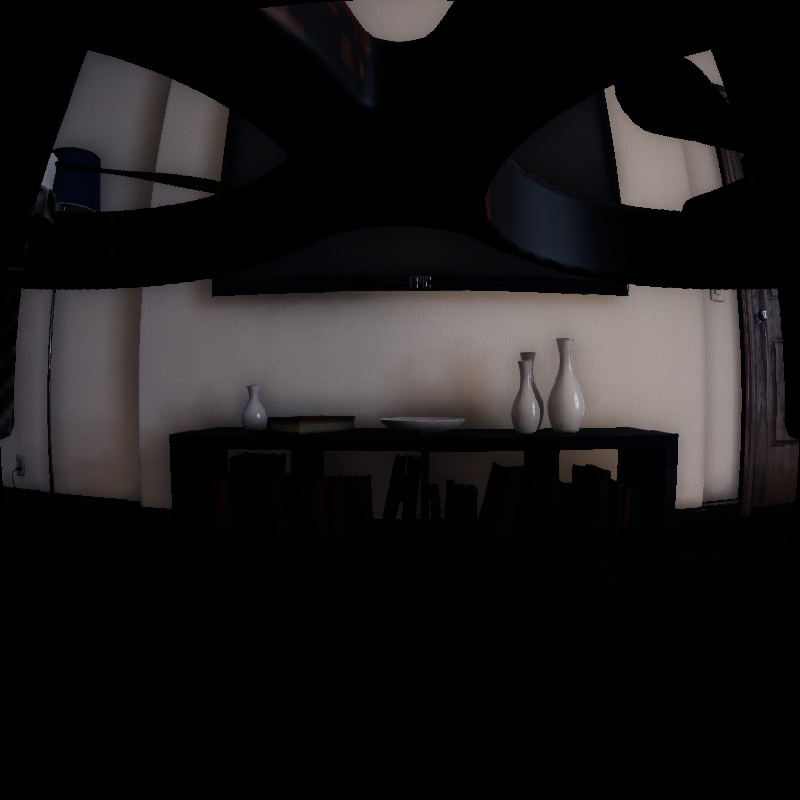
\includegraphics[height=6cm]{rapport/fig/Results/single/single_equi_distort_noline.jpeg}
        \caption{$r(\phi) = 1.0 \cdot \phi$}
        \label{fig:res_different_distortion_k1}
    \end{subfigure}
    \begin{subfigure}{0.45\textwidth}
        \centering
        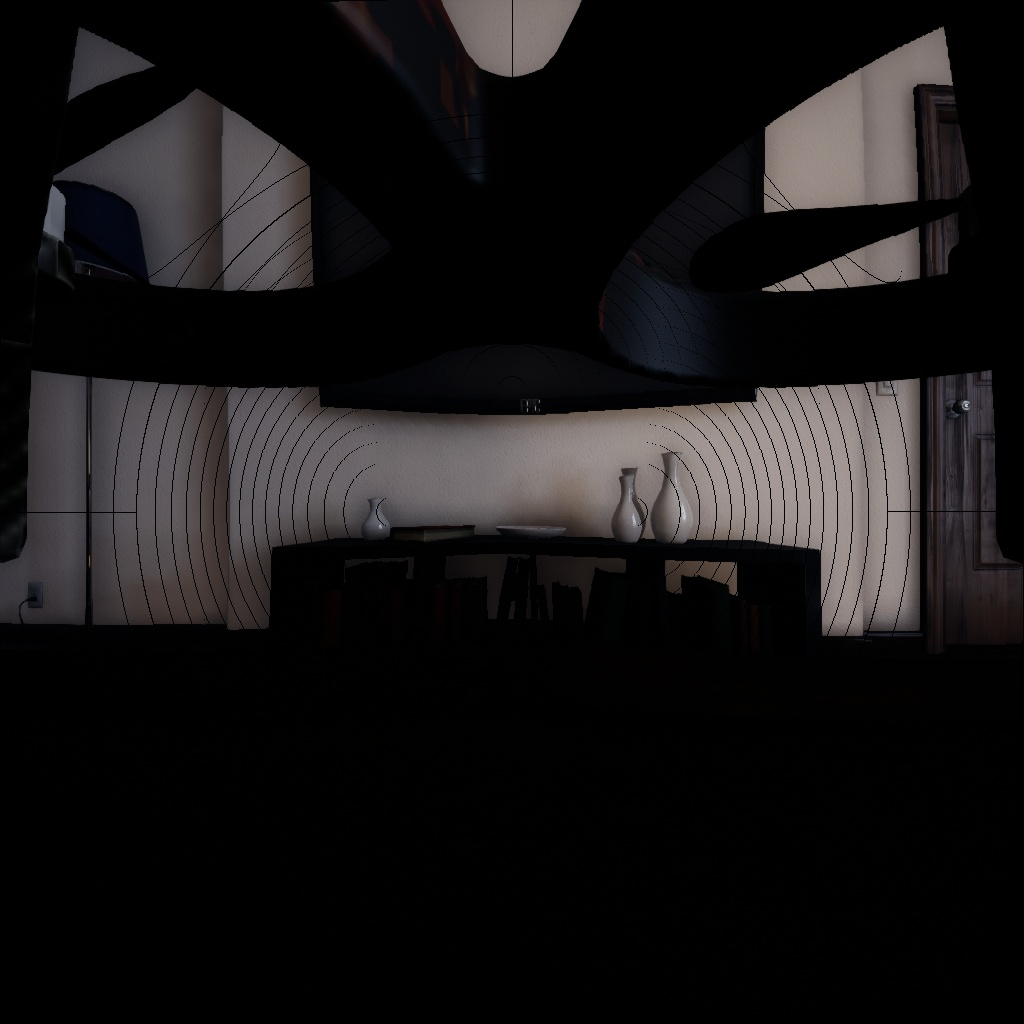
\includegraphics[height=6cm]{rapport/fig/Results/single/single_k2_distort.jpeg}
        \caption{$r(\phi) = 1.0 \cdot \phi + 0.7 \cdot \phi^2 + 0.3 \cdot \phi^3$}
        \label{fig:res_different_distortion_k1k2k3}
    \end{subfigure}
    \caption{Single pictures taken from the frontal camera using different distortion models}
    \label{fig:res_different_distortions}
\end{figure}

Figure~\ref{fig:res_different_distortion_k1k2k3} also shows significant distortion lines in the pictures. As with Figure~\ref{fig:res_comp_equal_512_1024}, this is caused by having too high resolution on the output image compared to the input image. However, for this example it shows the principle of nonlinear radial distortion, where the contour lines have increased spacing, with increasing $\phi$.

\subsection{Captured camera effects}

Refering to Table~\ref{tab:comparison_camera} and Table~\ref{tab:comparison_shader}, different camera lens and shader effects supported by Unreal Engine were presented. These effects appear as natural phenomenon in captured images. Table~\ref{tab:res_shader_effects} sums up the various tests, showing whether the functionality is Supported and actiavtable through AirSim, and or supported by the fisheye camera module. The column for Last colums represents the ability to easilly tweak the simulations directly in the Unreal Engine editor, before simulation start.

\begin{table}[!htb]
    \centering
    \begin{tabular}{|c|c|c|c|c|} \hline
        \textbf{Effect} & Fisheye camera & AirSim & AirSim tweakable & UE4 tweakable \\ \hline \hline
        Automatic exposure & Yes & Yes & Yes & Yes* \\ \hline                 
        Manual shutter speed & No* & No* & No & Yes \\ \hline
        Motion Blur & No & No & No & No \\ \hline
        Lens Flares & Yes & Yes & No & Yes \\ \hline
        Light shafts & \multicolumn{2}{c|}{Not tested} & No & Yes* \\ \hline
        Bloom & \multicolumn{2}{c|}{Not tested} & No & Yes* \\ \hline
        Chromatic aberration & \multicolumn{2}{c|}{Not tested} & No & Yes* \\ \hline
        Vignette & No & No & No & Yes* \\ \hline
        Natural shadows & Yes & Yes & No & Yes \\ \hline
        Ambient occlusion & \multicolumn{2}{c|}{Not tested} & No & Yes* \\ \hline
        Reflections & Yes & Yes & No & Yes \\ \hline
        Noise & Some & Yes & Yes & Yes \\ \hline
        
    \end{tabular}
    \caption{System overview of supported shader effects. (*) marked entries are explained futher in this section.}
    \label{tab:res_shader_effects}
\end{table}

The exposure settings are controllable through the AirSim settings. This does not include the manual override of the automatic eye adaption mechanic of Unreal Engine. However, minimum, maximum exposure as well as adaptation speed can be controlled freely. This means that the simulator does not support setting a specific exposure time or shutter speed directly. The settings for manual shutter control can be set directly in the Unreal Engine editor, by turning off the eye adaptation mechanic. This enables manual shutter speed for both AirSim and the fisheye camera. It is stated by the developers of AirSim that motion blur is implemented. However, it has not been functioning in any of the tests. Further investigation is needed, as there may be other post processing elements overwriting this setting.

The shader effects shown in Table~\ref{tab:comparison_shader}, are in many cases integrated into the images shown in the results. Looking closely at Figure~\ref{fig:res_show_fisheye}, it can be seen that shadows are cast from the picture frames and the sofa, caused by the spot lights on the wall. We also see the that the railings, curtains and door frame cast realisticly looking shadows, based on the outdoor lighting. One special thing to note here is the part of the curtains in direct sunlight does not soften the shadow cast on the floor, even though much of the light passes through it, showing some of the shaders deficiency. It is possible to recreate these effects, with additional artificially placed light sources.

Many effects has to be set up manually in the scnene editor to make work correctly. One of these is Reflections. Reflections are clearly shown in Figure~\ref{fig:res_comp_single_2048_1500}, captured on the vase, meaning that it transfers to the fisheye camera without any problems. Vignete, lens flare, light shafts, bloom and chromatic aberration, are post processing effects that are not directly available through AirSim. These needs to be directly enabled in the Unreal Engine editor for each specific scene and capture component. However, it is not known whether AirSim will interfere with these mechanics. Vignette is currently not supported by the fisheye camera, as it appears as five rings in the transformed image. The others are not specifically tested, but lens flares can be seen in Figure~\ref{fig:res_show_fisheye}, where it gets distorted as is expecteed by non-radial lens flares.

Noise is a problem for the simulator. While the effects are shown, they are applied to the original perspective images before they are transformed. This means that especially wave distortion will appear to be stretched out in the image, as seen in Figure~\ref{fig:res_pp_noise_yes}. Reduced noise effects can still be applied with reasonable functionality, but the settings has to be fine tuned, and may suddenly produce unintentional artifacts, especially with random noise settings applied.

\subsection{Performance} \label{sec:res_performance}

While the performance never was a part of the equation when implementing it, it is an important factor in a control application. All tests have been performed on the office PC in at NTNU. This PC does not have a dedicated graphics card, and Unreal Engine lagged considerably during tests. How much this affected the tests is unknown. however they should show qualitative data to shed some light upon areas to imporve the simulator.

Table~\ref{tab:res_timing_single} and \ref{tab:res_timing_cube_capture} show the timings in seconds for different resolutions and capture types. Note that while this is not even close to real time, all calculations done by the simulator are done sequentially for each pixel in the picture, meaning that no parallellization has been done. This can clearly be seen by comparing the calculation times, where the computation time follows the increase in resolution linearly. The fetch times are also higher for higher resolution picture, which are to be expected. Around $512\times 512$ it became quite noticable. 

\begin{table}[!htb]
    \centering
    \begin{tabular}{|c|c|c|c|} \hline
        \textbf{Input resolution} & \textbf{output resolution} & \textbf{Timing type} & \textbf{Time elapsed} \\ \hline \hline
        \multirow{2}{*}{$256 \times 256$} & \multirow{2}{*}{$512 \times 512$} & Fetch & 0.1 - 0.2 s \\ \cline{3-4}
         & & Transform & 0.4 s \\ \hline
        \multirow{2}{*}{$512 \times 512$} & \multirow{2}{*}{$512 \times 512$} & Fetch & 0.1 - 0.2 s\\ \cline{3-4}
         & & Transform & 1.5 s \\ \hline
        \multirow{2}{*}{$1024 \times 1024$} & \multirow{2}{*}{$1024 \times 1024$} & Fetch &  0.3 - 0.5 s \\ \cline{3-4}
         & & Transform & 6.0 s \\ \hline
        \multirow{2}{*}{$2048 \time 2048$} & \multirow{2}{*}{$2048 \times 2048$} & Fetch & 0.6 - 0.7 s\\ \cline{3-4}
         & & Transform & 24.1 s\\ \hline
    \end{tabular}
    \caption{Timing for single capture transformation to fisheye image}
    \label{tab:res_timing_single}
\end{table}

\begin{table}[!htb]
    \centering
    \begin{tabular}{|c|c|c|c|} \hline
        \textbf{Input resolution} & \textbf{output resolution} & \textbf{Timing type} & \textbf{Time elapsed} \\ \hline \hline
        \multirow{2}{*}{$256 \times 256$} & \multirow{2}{*}{$256 \times 256$} & Fetch & 0.3 - 0.4 s\\ \cline{3-4}
         & & Transform & 2.0 s\\ \hline
        \multirow{4}{*}{$512 \times 512$} & \multirow{2}{*}{$512 \times 512$} & Fetch & 0.4 - 0.5 s \\ \cline{3-4}
         & & Transform & 7.9 s\\ \cline{2-4}
         & \multirow{2}{*}{$1024 \times 1024$} & Fetch & 0.4 - 0.5 s\\ \cline{3-4}
         & & Transform & 7.9 s\\ \hline
        \multirow{2}{*}{$1024 \time 1024$} & \multirow{2}{*}{$1024 \times 1024$} & Fetch & 0.7 s\\ \cline{3-4}
         & & Transform & 30.9 s\\ \hline
    \end{tabular}
    \caption{Timing for cube capture transformation to fisheye image}
    \label{tab:res_timing_cube_capture}
\end{table}


\section{Discussion}

Both the $360^\circ$ image capture simulator and the ROS publisher node has been implemented, and is working for their intended purposes. There are however still a lot of details that needs to be sorted out for this to be a releasable product. The main issue is the performance, in the form of time delay, where a control application running on this simulator needs to get the video feed at a reliable rate in order for the simulator to appear as though it was a real system. Another is usability and available customization, where the simulator should provide the option to add this camera type to different vehicles, different configurations for the multirotor.

On the other hand, the simulator provides great image qualities with lighting effects that are hard to create in other simulators. Effects like the occlusion created on other objects when the camera is exposed to direct sunlight are effects that CV-algorithms have to deal with, but there are limited resources for simulating accurately. Using this simulator, new data sets can be made by recreating environments or just flying along new paths. This is especially powerful for deep learning application, where over-fitting to a small sample size is a common problem. This chapter will discuss these topics in more detail, reflect upon the choices made, and present further work and advancement opportunities for the simulator. 

\subsection{Platform}

The Unreal Engine platform was chosen because of the face that its powerful rendering and shading capabilities would add many realistic effects, that are not available in many other simulators, while still being largely important problems to solve in CV algorithms. As powerful graphics cards and computer processing power become more and more available, this would also be able to enable the simulator to be long term sustainable. The fact that it already had available simulators for both CV and vehicle simulations already implemented through AirSim, meant that the project could be fully focused on the implementation of the fisheye camera. As there are no other omnidirectional camera simulators available, this was a reasuring element.

The largest problem with Unreal Engine is also its strength. There are so many tools and so many features added, which all influence each other in different ways, that it is really hard to get a good overview of the system and the editor. This would not have been that much of a problem in Gazebo, where the simulator in many ways are more specialized to its task. Gazebo also provides a modular modeling system that is much closer to that of mathematical modeling, while the same functionality can be found in Unreal Engine, it is often hidden behind many different abstractions and tools, which make sense when making a game. It is also these abstractions that enables the platform to produce high quality graphics, while still running in real time.

Choosing gazebo might have been more time efficient, and would probably have meant that the camera module had been implemented faster, allowing for additional testing and comparisons with real camera setups and calibration techniques. There are also quite many vehicle models already implmented in Gazebo, which could have been used in these experiments, in the same way that AirSim provides. Using AirSim or similar platforms for Gazebo would most likely amount to about to the same workload. However, AirSim has the advantage of implementing a lot of sensors in one package, which has been tried and tested to work together.

\subsection{Implemntation}

Towards the end of the project the module was changed to become a client based module, instead of working as a Part of AirSim. This choice was made, looking at the progress, and the amount of change that was necessary in order to get the module up and running. While this made the platform significantly easier to develop, it also removed the possibility of using many of the advanced features of Unreal Engine. This mainly affects the performance of the module, which will be discussed in Section~\ref{sec:disc_performance}. It also changes the way the module had to be implemented.

While the cubemaps of Unreal Engine in itself incorporate the same basic structure as the fisheye tranformer module does, the cubemaps of Unreal Engine are optimized and integrated with the toolset. Most importantly the cubemaps provide the the functionality to render without post-processing effects on, which means that extra effects that should not be modified by the lens distortion, can be added after the transformation.

The usage patterns of the module also changes quite a bit. The fact that it is split completely from AirSim and Unreal Engine means that it will not affect either of these, if it is not used. It is disabled by simply not including the header file to the specific test application. The only dependencies include the camera setup on the vehicle model in Unreal Engine, and the camera attatchment and naming script in AirSim. These needs to be set individually for all AirSim projects and vehicles, which is why they are not counted as direct dependencies.

In retrospect, the RPC server/client dependency of the ROS publisher could also have been avoided completely. While it provides a simple way for making clients to control AirSim in other programming languages than C++, it is not needed as this is a full C++ project. it only adds complexity and possibly also some latency.

Because of these reasons, and in order to make a releasable simulator, it would be best to apply this module to AirSim directly, and having it managed by Unreal Engine game mode. This way there would be much more oppurtunities for optimization, as well as the fact that both the tranformer and ROS publisher would be completely independent of the RPC server/client service.

\subsection{Image Quality and captured effects}

While image quality and level of detail in the picture is important, it does often have to be disregarded in control applications due to the time it takes to extract information from large images. Even though this is to some extent less relevant for large moving vehicles like cars and ships, where one can store hardware capable of high amounts computation power, it is highly relevant for smaller objects like the multirotor in this simulator or other small vehicles. However, this does not mean that advanced shader effects, such as reflections are removed. Rather these effects tend to blend into the object coloring, creating even more difficulties for the CV application. This effect can clearly be seen in Figure~\ref{fig:res_comp_single_256_200}, where the reflections of the curtain is still apparent in the vases on the table. However the textures are harder to discern from each other, since less of the contrast is captured.

When it comes to the distortion mapping, the fisheye camera does its job well. The total picture is best shown in Figure~\ref{fig:res_show_fisheye}, and here we clearly see that there are no mismatching textures, or lines resembling the stitching of the images. This would probably have been most apparent in the balcony door, where there is a stitching between the front and downwards pointing camera. It also produces the expected radially increasing distortion effect, and ends up as a circular image on the image plane, as it would with a real fisheye camera. Looking at the original pictures in Figure~\ref{fig:res_original_pictures}, it can be seen that all light and shadow effects have been correctly mapped into the new image, as these effects are also prone to the lens distortion. 

In low resolution pictures, as seen in Figure~\ref{fig:res_comp_256_to_256}, the pictures become highly pixelated. This effect is caused by the way the mapping algorithm chooses the final color of the pixel, where it will draw that last color mapped to that specific pixel. A solution to this would be to implement anti-aliasing techniques, in the cases where this happens. This should be implementable without introducing too complex computations or time delays. Whether or not it is necessary is however uncertain, as the problem is removed for resolutions around $500\times 500$ pixels and upwards. There are also very few high FoV fisheye cameras with this low resolution, which would imply that the problem is insignificant.

Another problem seen in the simulator comes when increasing the resolution of the output picture beyond the resolution of each individual perspective picture. Since the images towards the edges of the picture gets stretched much more than the center parts, there are not enough pixels in the original image to map to these points. The effects are seen in Figure~\ref{fig:res_comp_equal_512_1024} and \ref{fig:res_different_distortion_k1k2k3}, where it looks like distortion lines are appearing. This effect would not appear in a real camera, as there would be a continous field of light hitting the whole lens. One solution to this may be capturing the horizontal perspective images with a higher resolution than the downward looking camera. Another solution would be to add gradient effects, mapping the outlier pixels with an average of the color of the pixels around it. 

The scaling introduced in Equation~\eqref{eq:impl_pixel_transform_final} is a way to ensure that the final picture fits the output resolution of the image. This provided an easy way to test the simulator. However it should not be active when calibrating the simulators camera to an actual fisheye camera, as it negates parts of the lens parameters physical relation. As an example, in the equidistant model $r=k_1 \phi$, the $k_1$ parameter directly ties to the focal length of the fisheye camera, mapping the fisheye projection to an image plane with a specific size. In that camera, the photosensitive CCD would also have physical dimensions which may or may not match the image plane. The scaling parameter, as it is proposed, would ensure that these match, providing incorrect results. In real calibration this scaling should be chosen relative to the size of each pixel on the CCD.

As the lens model is now, it only incorporates radial distortion in the images. In a real camera one may encounter off center distortions, image stretching due to misalignment of the lens and image plane, tangential distortion or any combinations of these. While the simulator does not incorporate them at this moment, the lens model is made to be changed easily, as it only implements its parameters and a simple distorting function, calculating the radius from center for the new pixel.

Many additional post processing effects are supported by Unreal Engine, which means that many effects that appear because of lens inaccuracies or natural phenomenons can be captured in the images. The main problem about this is that it is applied to the perspective images, and not to the fisheye image directly. This means that effects that should not gain additional distortion, such as some effects of noise in the image. However, most effects that are light based, like reflection, refraction, shadowing and direct light, will appear as they should in the converted image. Though this has not been specifically tested for all effects, there is considerable evidence in the presented pictures supporting this claim.

When it comes to exposure settings, shutter speeds, the effects of these as well as noise, are of the most important effects to capture in the simulator. While most cameras have an automatic exposure function, it can be beneficial to manually control this for certain experiments and algorithm tests. AirSim currently only implements control over the eye adaptation mechanic in Unreal Engine. This allows control of maximum and minimum exposure, as well as adaptation speed and bias, directly from the AirSim settings. In order to gain control of the shutter speed, the camera settings in unreal needs to be set to manual mode. This provides control for Shutter speed, aperture and ISO value. While the exposure settings worked great, as shown in Figure~\ref{fig:res_pp_exposure_yes}, the motion blur does not work. None of the camera overrides in Unreal Engine did fix this. It may be caused by AirSim overwriting the settings while it is running.

Additional noise can be added through, with many tunable parameters including randomness, density, strength, how many pixels share the noise, different patterns and so on. The effects work really well for perspective images. Transforming the pictures does unfortunately not handle this well, as the noise gets stretched out, especially towards the edges of the image. As noise is not a direct light based effect, the same distortion should not apply to it. While the noise contribution added in AirSim is applicable for minor amounts of noise, this should be added to the picture after transformation. This is not possible with the current version of the simulator.

\subsection{Performance and optimization} \label{sec:disc_performance}

As described in Section~\ref{sec:res_performance}, the operational speed of the tranformer is quite slow. Ranging from 2 seconds per picture for the low $256\times 256$ pixel resolution, up to 31 seconds for $1024 \times 1024$ pixel pictures. This is caused mainly by the fact that the complete sequance of transformations descibed in Chapter~\ref{chap:simulator} is repeated for every pixel in the image. Looking at the table, we also see a linear increase in computation time with the amount of pixels in the image. This is because each pixel transformation is computed sequentially.

Since both the rotations of the perspective images and the distortion calculations are completely static, as long as neither the FoV or the resolution changes, the all calculations can be done as a part of the start up routine of the simulator. By saving the pixel mapping for all five source images, all further transformation may be done in linear time. Even though this removes the most demanding calculations from the real time task of the simulator, the startup time of the simulator scales too badly, and parallelization should therefore be applied.

The transformation itself is a highly paralellizable task, where the only common writing operation is the output picture, or the mapping matrix in this case. This process would also be free of race conditions as each thread would work on it's own pixel calculations and writing it to its own space in the mapping matrix. because of the amount of pixels in the picture is as high as it is, it would be optimal to make use of a GPU library like CUDA or OpenCL for these calculations.

The fetch times are also too long and inconsistent, which might be a harder problem to solve. It is either caused by the message packaging of the RPC system, or it is caused by the way AirSim handles the image captures. The RPC client is in many ways an unnecessary slowing element in the implementation, as the communication between the server and client uses a serialized TCP/IP connection. This means that it could possibly apply a bottleneck in the computation pipeline.

Removing the dependency on the RPC client would mean that the fisheye and ROS client would need modifications, making them applicable to run inside an Unreal Engine game loop. The best way to implement this would probably be to redesign the module in order to use Unreal Engines Matrix and Image types, which are already optimized for graphics computing. Adding the module to the game loop would also benefit the user of the simulator, as they would only have to deal with one start button for the simulator. 


\cleardoublepage